\section{仿生机器鼠正运动学}
机器鼠模型具有11个主动自由度,其配置情况如图\ref{figure_kinematic}\subref{figure_dof}。除轮部运动外,机器鼠的动作规划主要涉及其中的臀部、腰部和头部的7个关节,相应的坐标系统如图\ref{figure_kinematic}\subref{figure_dhframe}。
\begin{figure}[htbp]
  %\vspace{13pt}
  \centering
  \subfigure[自由度配置\cite{liDesignOptimizationLightweight2020}]{
  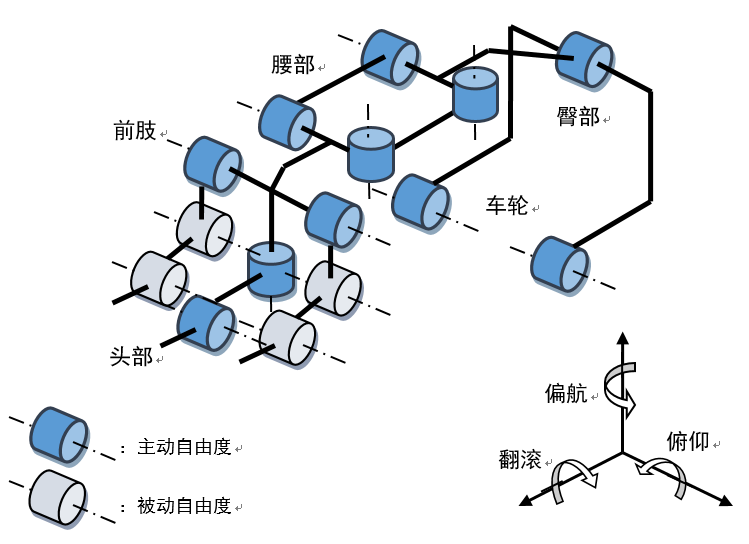
\includegraphics[height=0.21\linewidth]{images/ch02/dof.png} \label{figure_dof}
  }
  \subfigure[坐标系统\cite{liMotionEvaluation2017}]{
  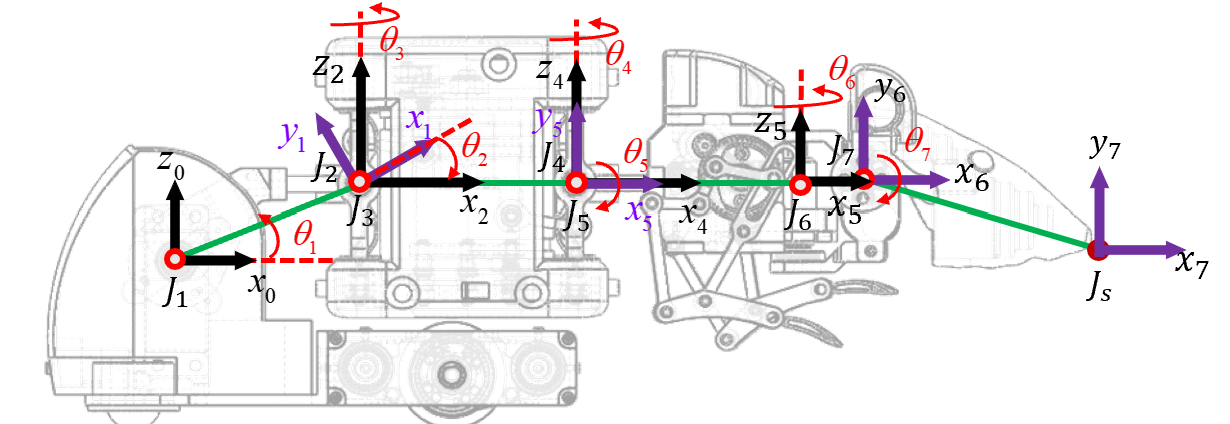
\includegraphics[height=0.21\linewidth]{images/ch02/dhframe.png} \label{figure_dhframe}
  }
  \caption{机器鼠模型自由度配置情况及其坐标系统}\label{figure_kinematic} % label 用来在文中索引
\end{figure}

七自由度机械臂的逆运动学求解是一大难点,在机械臂结构设计非特殊的情况下,通过迭代方法求得数值解是其通用解法\cite{shimizuAnalyticalInverseKinematic2008}。而考虑到数值解需要一定的计算时间,而这与实时行为交互所需的快速性相违背,因此通过正运动学计算设计特定的动作,直接控制其关节位置,而不是通过逆运动学求得关节位置,将能够显著降低程序计算时间,并提高行为交互的实时性。
%\begin{figure}[htbp]
%  \vspace{13pt}
%  \centering
%  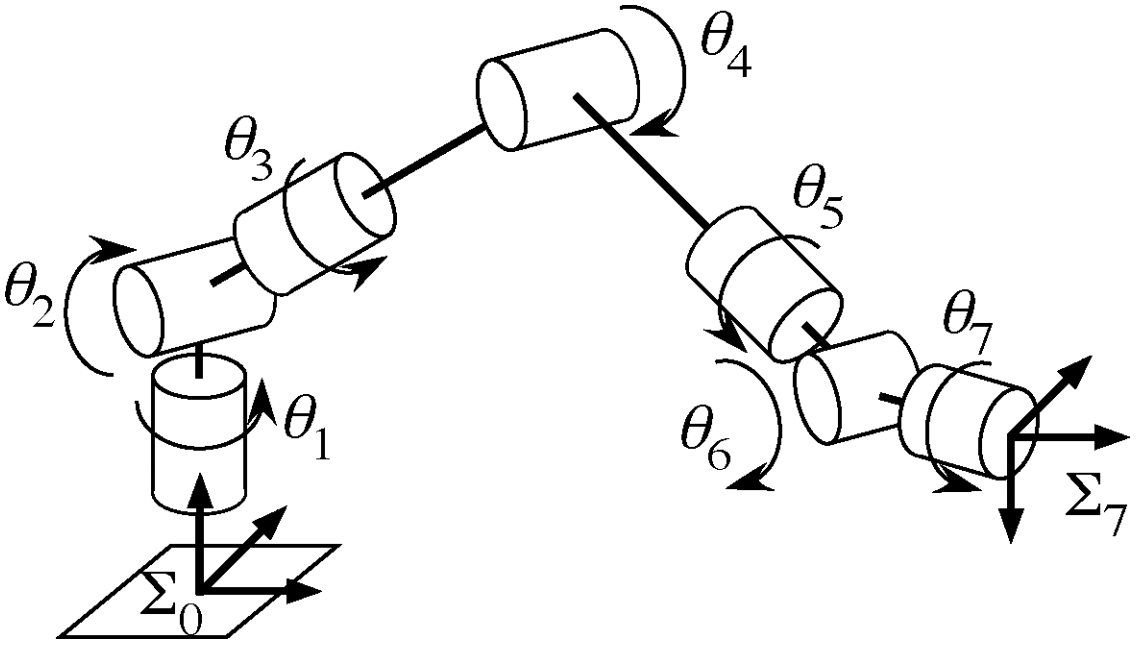
\includegraphics[width=0.6\linewidth]{images/ch02/7dof.png}
%  \caption{S-R-S构型七自由度机械臂\cite{shimizuAnalyticalInverseKinematic2008}}\label{figure_7dof}
%\end{figure}

对生物鼠而言,头部既是其重要的感知和决策部位,包括视觉、听觉和嗅觉等多种主要感觉器官和大脑这一神经中枢;又是其重要的动作执行器,几乎全部动作都需要头部的参与,并且其嘴、鼻等重要的动作执行器官也位于这一区域。因此,保证机器鼠头部的工作空间与生物鼠相同,能够为其产生仿鼠动作提供必要条件。

计算仿生机器鼠头部工作空间属于机器人正运动学的范畴,通过列写相邻关节的变换矩阵获得。根据图\ref{figure_dhframe},可以建立机器鼠躯干部分的D-H连杆参数表为表\ref{table_dh}。
\begin{table}[htbp]
  \linespread{1.5}
  \zihao{5}
  \centering
  \caption{机器鼠躯干部分D-H参数表}\label{table_dh}
  \begin{tabular}{*{5}{>{\centering\arraybackslash}p{2cm}}}
    \toprule
    $i$ & $\theta_i$ & $\alpha_{i-1}~(deg)$ & $d_i~(m)$ & $a_{i-1}~(m)$ \\ \midrule
    1   & $\theta_1$ & 0   & 0 & 0.058 \\
    2   & $\theta_2$ & -90 & 0 & 0     \\
    3   & $\theta_3$ & 0   & 0 & 0.033 \\
    4   & $\theta_4$ &  90 & 0 & 0     \\
    5   & $\theta_5$ & -90 & 0 & 0.04  \\
    6   & $\theta_6$ & 90  & 0 & 0.04  \\
    7   & $\theta_7$ & 0   & 0 & 0.012 \\
    \bottomrule
    \end{tabular}
\end{table}

而利用D-H法求解机器人正运动学的相邻坐标系间的变换矩阵为式\ref{equation_transfer},式中$1 \leq i \leq 7,i\in \mathbb{Z}$。对串联机器人而言,$\prescript{0}{7}{T}=\prod_{i=1}^{7}\prescript{i-1}{i}{T}$,可以计算得到机器鼠头部与其基座的变换矩阵,利用计算机可以加速这一过程。
\begin{equation}\label{equation_transfer}
  \prescript{i-1}{i}{T}=\left[\begin{array}{cccc}
        c\theta_{i} & -s\theta_{i} & 0 & a_{i-1} \\
        s\theta_{i}c\alpha_{i-1} & c\theta_{i}c\alpha_{i-1} & -s\alpha_{i-1} & -d_{i}s\alpha_{i-1} \\
        s\theta_{i}s\alpha_{i-1} & c\theta_{i}s\alpha_{i-1} & c\alpha_{i-1} & d_{i}c\alpha_{i-1} \\
        0 & 0 & 0 & 1
  \end{array}\right]
\end{equation}

机器鼠躯干部位各个关节的运动范围为表\ref{table_jointlimit},利用matlab在其关节空间中生成10000个点,构成机器鼠头部的运动空间,如图\ref{figure_workenv}所示,其计算脚本为\ref{appendix_wsscripts}。
\begin{table}[htb]
  \linespread{1.5}
  \zihao{5}
  \centering
  \caption{机器鼠关节限位}\label{table_jointlimit}
  \begin{tabular}{p{6cm}<{\centering\arraybackslash}p{2cm}<{\centering\arraybackslash} p{2cm}<{\centering\arraybackslash}}
    \toprule
    关节                                       &  $min(rad)$ & $max(rad)$  \\ \midrule
    $base\_to\_body\_link1\_joint$  &  -1  & 0  \\
    $body\_link1\_to\_link2\_joint$ &  -0.5  & 0.5 \\
    $body\_link2\_to\_link3\_joint$ &  -0.6 & 0.6   \\
    $body\_link3\_to\_link4\_joint$ &  -0.6 & 0.6 \\
    $body\_link4\_to\_link5\_joint$ &  -0.5 & 0.5 \\
    $body\_link5\_to\_link6\_joint$ &  -0.5 & 0.5 \\
    $body\_link6\_to\_head\_joint$  &  0 & 0.3 \\
    \bottomrule
    \end{tabular}
\end{table}
\begin{figure}[htbp]
  %\vspace{13pt}
  \centering
  \subfigure[前视]{
  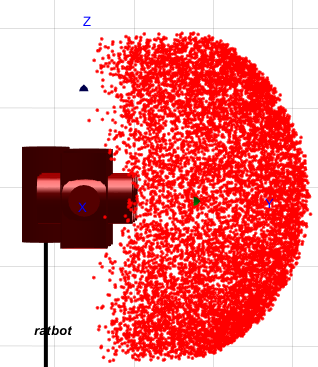
\includegraphics[height=0.25\linewidth]{images/ch02/workenv/front.png} \label{figure_workenv_front}
  }
  \subfigure[侧视]{
  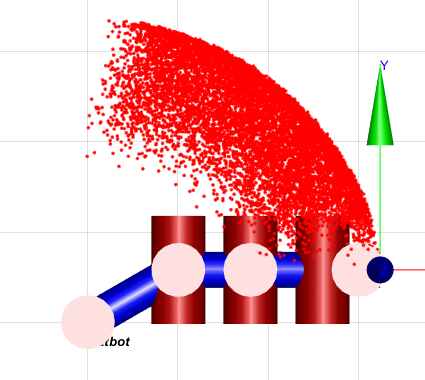
\includegraphics[height=0.25\linewidth]{images/ch02/workenv/left.png} \label{figure_workenv_left}
  }
  \subfigure[俯视]{
  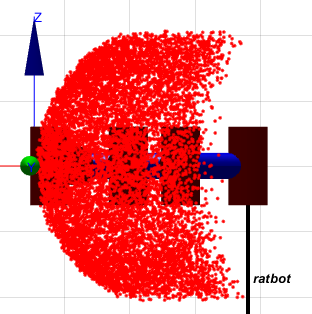
\includegraphics[height=0.25\linewidth]{images/ch02/workenv/top.png} \label{figure_workenv_top}
  }
  \caption{机器鼠模型的头部工作空间}\label{figure_workenv}
\end{figure}

比较机器鼠头部工作空间和生物鼠头部的运动范围即可判断机器鼠能否执行相应的仿鼠动作。\citeauthor{liMotionEvaluation2017}重点比较了机器鼠和生物鼠在进行攀爬和梳理两种动作时的头部运动轨迹及相应的工作空间(图\ref{figure_comparetrace}),图中,BL(\underline{B}ody~\underline{L}ength)表示生物鼠或机器鼠的体长,蓝色箭头曲线为生物鼠头部运动轨迹,黄色箭头曲线表示机器鼠头部运动曲线,灰色部分为机器鼠工作空间\cite{liMotionEvaluation2017}。可以看出,生物鼠的头部运动轨迹均位于机器鼠的工作空间内部,因此机器鼠模型可以保证执行相应的仿鼠动作。
\begin{figure}[htbp]
  %\vspace{13pt}
  \centering
  \subfigure[攀爬]{
  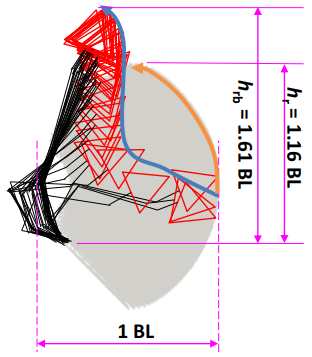
\includegraphics[height=0.40\linewidth]{images/ch02/workenv/mount.png} \label{figure_comparemount}
  }
  \subfigure[梳理]{
  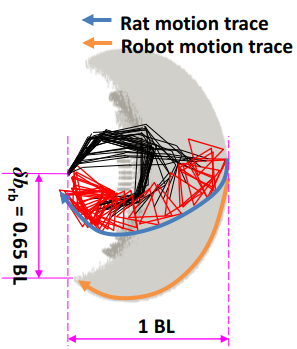
\includegraphics[height=0.40\linewidth]{images/ch02/workenv/groom.png} \label{figure_comparegroom}
  }
  \caption{机器鼠与生物鼠头部运动轨迹比较\cite{liMotionEvaluation2017}}\label{figure_comparetrace}
\end{figure} 